\documentclass[11pt,a4paper,onecolumn]{report}
\usepackage{amsmath}
\usepackage{mathtools}
\usepackage{lmodern}
\DeclarePairedDelimiter{\abs}{\lvert}{\rvert}
\usepackage{bm}
\usepackage[margin=2cm]{geometry}
\usepackage{array}
\usepackage{physics}
\usepackage{amssymb}
\usepackage{textcomp}
\usepackage[T1]{fontenc}
\usepackage{gensymb}
\usepackage{graphicx}
\usepackage{fancyhdr}
\pagestyle{fancy}

\usepackage{tikz}
\usetikzlibrary{shapes.geometric, arrows, calc}
\usepackage[nottoc, numbib]{tocbibind}
\tikzstyle{cool} = [rectangle, rounded corners, minimum width=3cm, minimum
height=1cm, text centered, draw=black, fill=gray!30, text width=3cm]
\tikzstyle{arrow} = [thick, ->, >=stealth]
\tikzstyle{line} = [thick, -, >=stealth]

\usepackage[detect-all]{siunitx}
\usepackage{breqn}
\usepackage{subfigure}
\usepackage{geometry}
\usepackage{listings}
\usepackage{caption}
\usepackage[utf8]{inputenc}
\usepackage{hyperref}
\usepackage{titlesec}
\usepackage[square,numbers,comma,sort&compress]{natbib}
\usepackage{upgreek}
\usepackage{aas_macros}
\usepackage{doi}
\usepackage{siunitx}
\usepackage{textgreek}


\geometry{a4paper, total={160mm,247mm}, left=25mm, top=25mm,}
\graphicspath{
 {figures/} }
\renewcommand{\listfigurename}{Figures}


\captionsetup{justification   = raggedright, singlelinecheck = false}

\hypersetup{colorlinks, citecolor=black, filecolor=black, linkcolor=black,
    urlcolor=black}

\renewcommand{\bibname}{References}

\bibpunct{(}{)}{;}{a}{}{,}

\hypersetup{
    colorlinks,
    citecolor=black,
    filecolor=black,
    linkcolor=black,
    urlcolor=black
}


\newcommand*\chem[1]{\ensuremath{\mathrm{#1}}}

\newcommand{\threevdots}{%
  \vbox{\baselineskip1ex\lineskiplimit0pt%
  \hbox{.}\hbox{.}\hbox{.}}}



% diagnose: Label(s) may have changed. Rerun to get cross-references right.
% \def\@testdef #1#2#3{%
%   \def\reserved@a{#3}\expandafter \ifx \csname #1@#2\endcsname
%  \reserved@a  \else
% \typeout{^^Jlabel #2 changed:^^J%
% \meaning\reserved@a^^J%
% \expandafter\meaning\csname #1@#2\endcsname^^J}%
% \@tempswatrue \fi}


%opening
\title{Thesis}
\author{Cameron Smith\\
Student ID: 28792912\\
Supervisors: Andrew Casey, Alina Donea}
\date{\today}



\begin{document}


\begin{titlepage}
  \begin{center}
    \vspace*{2cm}
    \Huge
    \textbf{Title of your Thesis}

    \vspace{2cm}
    \LARGE
    \textbf{Cameron Smith}

    \vspace{0.8cm}
    \Large
    \textit{Supervisors:}\\
    Andrew Casey\\
    Alina Donea

    \vfill
    \large
    An honours thesis presented for the degree of\\
    Bachelor of Science Advanced - Research (Honours)

    \vspace{0.3cm}
    \includegraphics[width=0.2\linewidth]{"Monash_Logo"}\\
    School of Physics and Astronomy\\
    Faculty of Science\\
    Monash University\\
    Australia

    \vspace{0.5cm}

    \today

  \end{center}
\end{titlepage}

\chapter*{Abstract}



\chapter*{Acknowledgements}

\tableofcontents


\listoffigures








\chapter{Introduction}




%
% Project outline from lit review
%

To train a cGAN to generate magnetograms from seismic maps, we require
a training set consisting of seismic maps and the corresponding magnetograms.
While the farside seismic maps are readily available\footnote{See
\url{http://jsoc.stanford.edu/data/farside/}.}, corresponding magnetograms are
not. However, not all hope is lost. The STEREO-A spacecraft is in a heliocentric
orbit that traverses the Sun relative to the Earth, allowing it to observe the
farside during some points of the orbit. While STEREO-A does not capture
magnetograms of the Sun, it does take EUV images which can be used to create
magnetograms by using a cGAN \citep{Kim2019}.\\

A small complication is that no data is available from when STEREO-A was
directly opposite the Earth (between March and July 2015), due to the
interference from the Sun. This limits the ability to get magnetograms that
exactly coincide with the farside seismic maps. To compensate for this, we can
match farside seismic maps with images taken by STEREO-A at an earlier (later)
time when it is behind (ahead of) the farside, such that the same `face' of the
Sun is imaged due to it's rotation. After generating the magnetograms from the
STEREO-A EUV images, we can create a dataset of seismic maps with the
corresponding magnetogram (albeit with some time difference). This process is
summarised in Figure \ref{fig:Project_summary}.\\



\begin{figure}
  \centering
  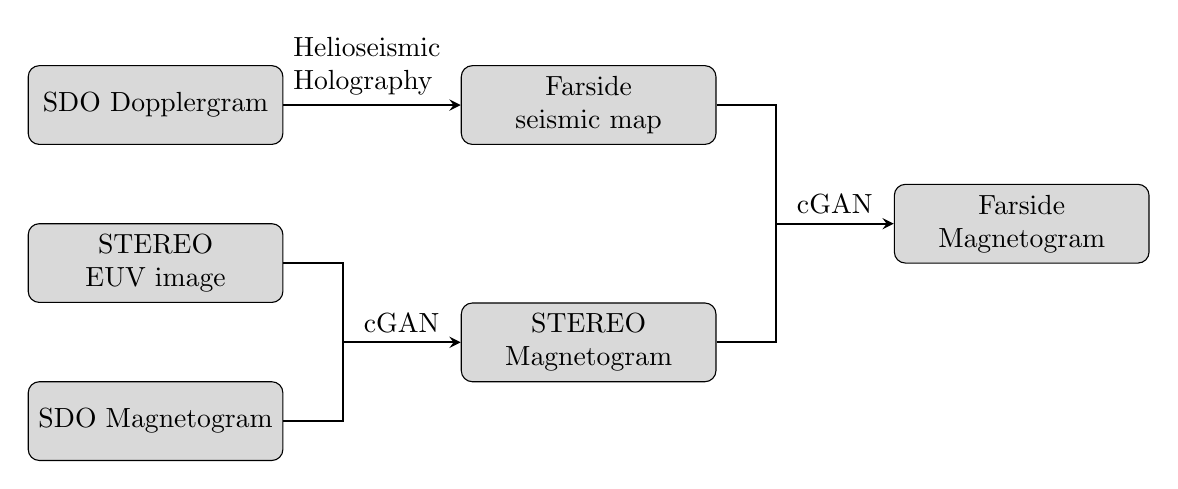
\begin{tikzpicture}[node distance=5.5cm]
      % \draw[help lines] (0,-5) grid (10,10);
      \node (D) [cool, above=1.5cm] {SDO Dopplergram};
      \node (P) [cool, right of=D] {Farside \quad \quad \quad \qquad  seismic map};
      \node (E) [cool] {STEREO EUV image};
      \node (M) [cool, right of=E, below=0.5cm] {STEREO Magnetogram};
      \node (F) [cool, right of=M, above=1cm] {Farside\\ Magnetogram};
      \node (S) [cool, below=1.5cm] {SDO Magnetogram};

      \coordinate (FF) at ([xshift=-1.5cm]F.west); % we collect the edges in front of Q
      \coordinate (MM) at ([xshift=-1.5cm]M.west); % we collect the edges in front of Q

      \draw [arrow] (D) -- node[anchor=south, text width=2cm] {Helioseismic Holography} (P);
      \draw [arrow] (MM) -- node[anchor=south] {cGAN} (M);
      \draw [line] (P) -|  (FF);
      \draw [line] (M) -|  (FF);
      \draw [line] (S) -|  (MM);
      \draw [line] (E) -|  (MM);
      \draw [arrow] (FF) -- node[anchor=south] {cGAN} (F);

  \end{tikzpicture}
  \caption{Summary of the project. A cGAN is trained on SDO data to be able to
  generate EUV images. This is applied to STEREO EUV images to generate STEREO
  magnetograms. These are used in conjunction with farside seismic maps to train
  a new cGAN to generate magnetograms from seismic maps, allowing constant
  surveillance of the farside magnetic field.}
  \label{fig:Project_summary}
\end{figure}



\chapter{Data Collection}
\begin{itemize}
  \item Data sources were:
  \begin{itemize}
    \item STEREO EUV images
    \item AIA EUV images
    \item AIA magnetograms
    \item farside helioseismic holography maps
  \end{itemize} 
\end{itemize}



\section{getting the stereo data}
- figure showing positions and tragectory of stereo, sun earth, SDO and
imaginary satelite for accoustic maps\\
- figure (maybe the same one) showing plot of stereo position in \\
- position data from http://www.srl.caltech.edu/STEREO/docs/position.html \\
-  This is in Heliocentric Earth equatorial (HEEQ): This system has its Z axis
parallel to the Sun's rotation axis (positive to the North) and its X axis
towards the intersection of the solar equator and the solar central meridian as
seen from the Earth. This system is sometimes known as heliocentric solar (HS)\\
- we want active regions to be at the same point of the image.\\
 - to do this, we have to compare stereo and accoustic maps taken at different
 times. \\
 - the sun has a period of T=27.2753 days according in carrington coordinates \\
 - angle between spacecraft and solar farside is given by: \\

\begin{align}
  \theta = \arctan{\frac{y}{x}}
\end{align}

- this gives:
\begin{align}
  t_{stereo} = t_{farside} + \frac{\theta}{2\pi}T
  \intertext{or equivalently:}
  t_{farside} = t_{stereo} - \frac{\theta}{2\pi}T
\end{align}
- using this, for each point in stereo time, i calculated the equivalent farside
time \\
- from this I download the FITS STEREO images that corresponded to the farside
images \\
 - (farside are created every 12 hours between 2010 and now)



\section{Data pre-processing}
- download the raw fits files of AIA and HMI from jsoc \\
- The FITS meta-data allows us to translate between pixel space and
helioprojective coordinate space.
- using this information, we can rotate the image such that the north pole is at
the highest point of the image, and then crop the image such that the edges of
the sun are at the edge of the image (see figure % From get_aia_png.ipynb
) \\

 - However the 304\AA \ channel of SDO AIA is degrading over time
 \cite{boerner_photometric_2014}, effectively reducing the exposure of the
 image. Figures \ref{fig:aia_degradation} show a comparison in the exposures of
 images taken in 2011, 2015 and 2019 respectively. To account for this
 degradation, the image was clipped to the 95th percentile of the pixel
 intensity and normalised. 


 \begin{figure}[t]%
  \centering
  \subfigure[]{%
    \label{fig:aia_2011}%
    \includegraphics[height=1.5in]{AIA_2011.01.01_00:00:00.png}% 
  }%
  \qquad
  \subfigure[]{%
    \includegraphics[height=1.5in]{AIA_2015.01.01_00:00:00.png}%
    \label{fig:aia_2015}%
  }%
  \qquad
  \subfigure[]{%
    \includegraphics[height=1.5in]{AIA_2019.01.01_00:00:00.png}%
    \label{fig:aia_2019}%
  }%
  \caption[]{
    Images taken by SDO AIA 304\AA \ on the first of January in
    2011 \subref{fig:aia_2011}, 2012 \subref{fig:aia_2015} and 2019
    \subref{fig:aia_2019}. Due to the degradation of the instrument, the
    exposure reduces over time. \textit{Images courtesy of NASA.}}
  \label{fig:aia_degradation}
\end{figure}





\section{Projections}
To train the GAN, features of the Sun need to be in the same position in both
the input and output training images.
The input image to the GAN, a seismic map, uses the projection


\bibliographystyle{mnras.bst}

\bibliography{Bibliography}


\appendix

\chapter{Coordinate Systems}
For a description of solar coordinate systems, see \citet{thompson_w_t_coordinate_2006}.


\chapter{just getting things down quickly}



\section{STEREO Magnetogram GAN}
- for the gan the input magnetograms and the seismic maps images needed to have
the same dimensions
- while the seismic maps were 180 by 180 pixels, the magnetograms were 1024 by
1024 pixels.

% currently thinking of upsampling seismic maps then downsampling magnetograms,
% but commented out paragraph shows my initial idea

% - to make them the same dimension, the magnetograms were resampled using bicubic
% interpolation to the size of the seismic maps. This interpolation method was
% chosen as it results in a smoother resampling with fewer interpolation artifacts
% \citep{keys_cubic_1981}.


- to make them the same dimension, the seismic maps were resampled using bicubic
interpolation to the size of the magnetograms. This interpolation method was
chosen as it results in a smoother resampling with fewer interpolation artifacts
\citep{keys_cubic_1981}.

 \end{document}

